\documentclass{article}
\usepackage[utf8]{inputenc}
\usepackage[colorlinks, allcolors=blue]{hyperref}
\usepackage{graphicx}



\title{Remote Sensing and GIS Integration Portfolio}
\author{Robert Vlasakker, van de}
\date{June 2021}

% Location of the images
\graphicspath{{figures/}}


\begin{document}


\maketitle

\section{Interactive Map I}
\textbf{Course Name \& Code.}
This interactive map was made for a master student that had trouble with Python Folium maps. 
So it has no specific course name and course code. 
It was for a master thesis internship for the study Forest and Nature Conservation.
\\

\noindent
\textbf{Description of the Application.}
The interactive map contains the location of cows over time as a heat map. 
Each cow had a GNNS sensor that reports the location every hour.
This map now shows the location of all the cows every hour. 
The time interval is set quite high as the sensors cover about three weeks of information (so the total amount of timestamps will be the amount of hours in three weeks.
\\

\noindent
\textbf{Description \& Requirements of Users.}
The potential users of the map were the master student and the viewers of the student's presentation.
The maps was used for a presentation to see how the cows moved through the park over time.
The watcher of the presentation were mostly managers of the park. 
This was a initial map to check to cows location. 
The main goal of the master internship was to locate high risk areas of the park.
A high risk area was defined as an area where cows and recreational users of the park were close.
\\

\noindent
\textbf{Purpose of your visualization.}
The purpose of the interactive map was to see how the cows moved over time through the park to get an initial idea where the cows were.
\\

\noindent
\textbf{Motivation for choice of visualization type.}
As the data contained time series an interactive map was the best choice. 
\\

\noindent
\textbf{Data sets.}
The dataset was a csv file containing 15666 rows and 17 columns.
An example of a part of the data can be found in Figure \ref{fig:csvfile}.
\\

\begin{figure}[ht]
    \centering
    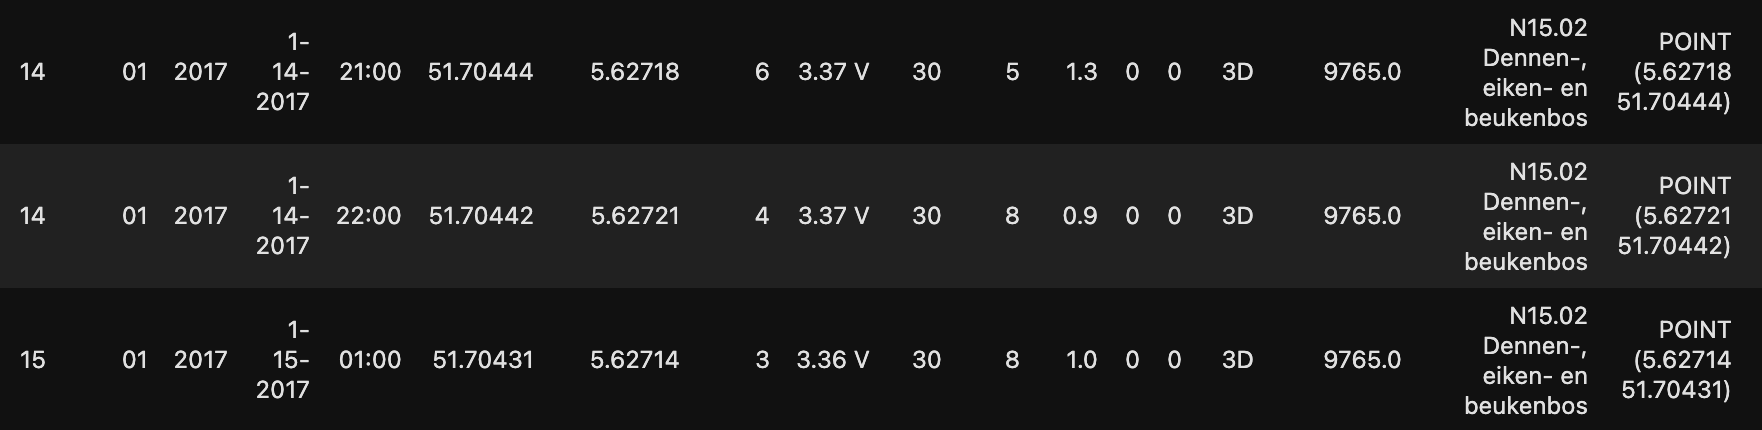
\includegraphics[scale=.4]{csv.png}
    \caption{Example of the data}
    \label{fig:csvfile}
\end{figure}



\noindent
\textbf{Data Processing.}
The Folium map was made using Python and several libraries.
Pandas/GeoPandas was used to read the csv file to read the geometry and the attributes.
Several data transformation were made to make the data more redouble for the Folium package.
All the points had to be grouped by their cow ID, so all the cow ID of a single timestamp could be plotted on the map.
The Jupyter Notebook (data not provided) containing all the code (including the saving of the map) can be found via this \href{https://github.com/RobertvdV/GRS60312_RemoteSensingAndGISIntergration_IDV_Portfolio/blob/master/notebooks/1.0-TimeStampFoliumMap.ipynb}{link}.
\\

\noindent
\textbf{Implementation.}
The final result can be saved as an HMTL file. This file can be opened on any computer/tablet/phone that has a browser.
The final result can be downloaded via this \href{https://github.com/RobertvdV/GRS60312_RemoteSensingAndGISIntergration_IDV_Portfolio/blob/master/data/processed/HeathMapPerDag.html}{link}.
\begin{figure}[h!]
    \centering
    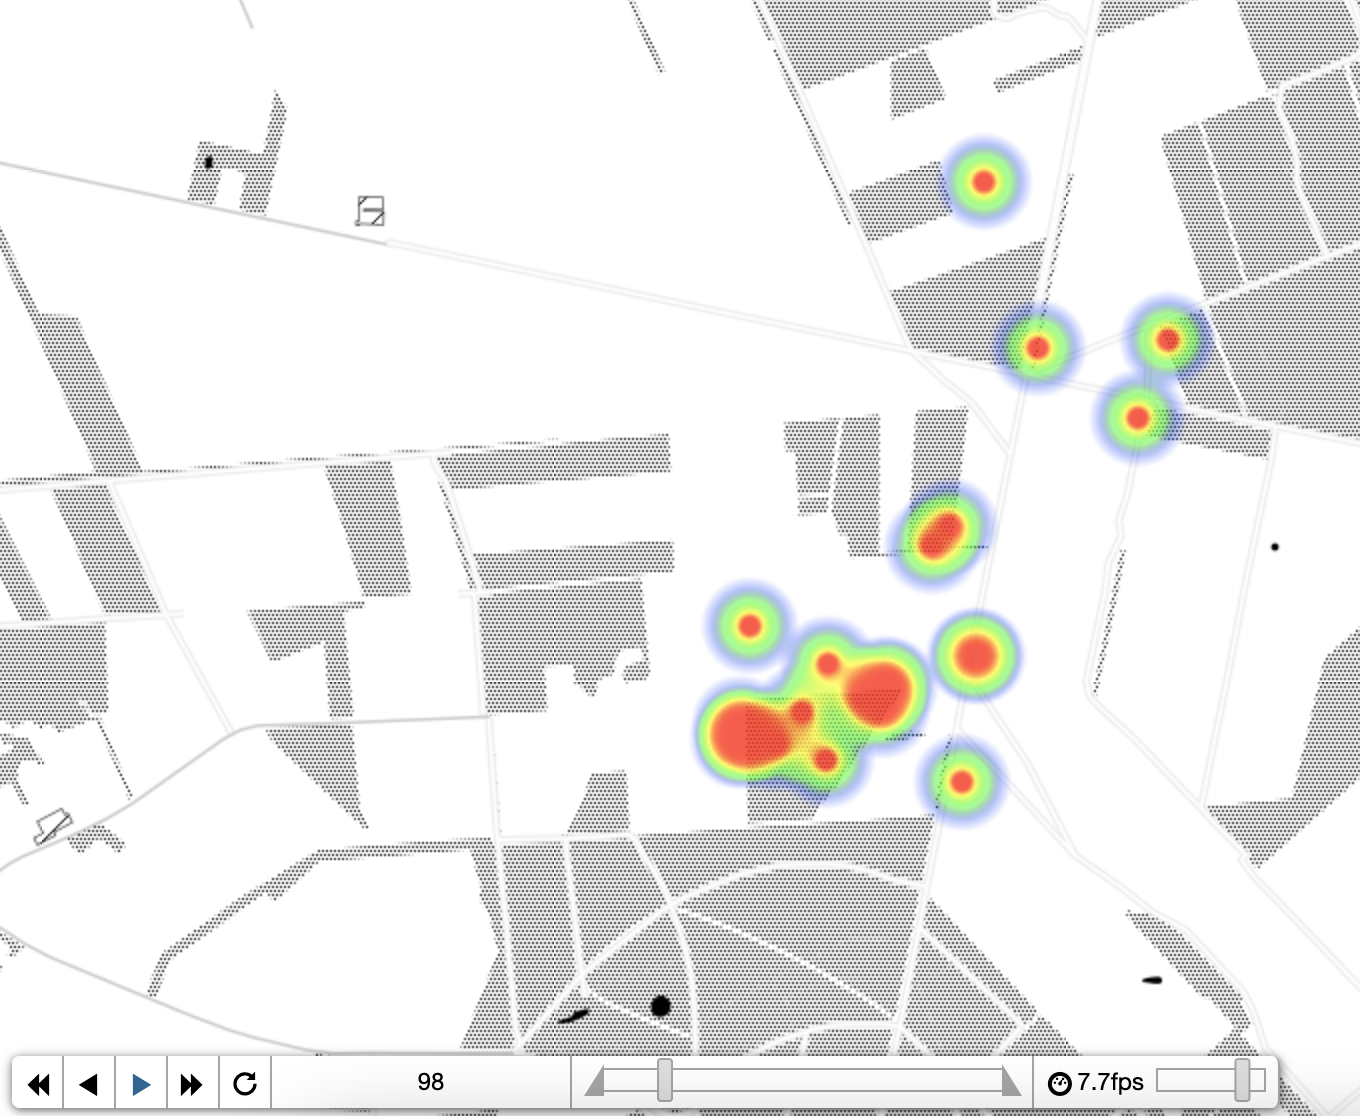
\includegraphics[scale=.35]{finalmap.png}
    \caption{Example of the final map}
    \label{fig:finmap}
\end{figure}

\noindent
\textbf{Reflection on the Result.}
As the \textbf{People} were all very satisfied, I think the map served the \textbf{Purpose} very well. 



\end{document}



